La funzione di ricezione dei campioni ha richiesto la definizione di una nuova \emph{API} di comunicazione con le applicazioni \emph{client} ed in seguito lo sviluppo delle componenti di manipolazione dei dati ricevuti per la relativa persistenza. Si presentano le specifiche tecniche e di implementazione di questi elementi.

\section{API}
Nel definire il dettaglio delle chiamate necessarie all'invio dei dati, si è valutato di prediligere i criteri di semplicità e adeguamento alle tecnologie attuali. Si è quindi optato per una \emph{API HTTP} e contenuto in formato JSON. La chiamata da utilizzare per l'invio dei dati risponde alla seguente specifica:

\begin{verbatim}
POST /api/data

BODY: 
{
    "type": "FeatureCollection",
    "features": [
        {
            "type": "Feature",
            "geometry": {
                "type": "Point",
                "coordinates": [
                    <longitude>,
                    <latitude>
                ]
            },
            "id": <unique_id>,
            "properties": {
                "timestamp": <timestamp>,
                "accuracy": <accuracy_value>,
                "labels": {
                    <label_name>: <label_value>,
                    ...
                }
            }
        },
        ...
    ],
    "properties": {
        "vote": <vote_number>
    }
}
\end{verbatim}
 Il formato definito consente di specificare una lista di elementi di campionamento e per ciascuno di esso le informazioni necessarie. Ogni campionamento è individuato da una chiave \emph{id} generata in modo casuale dal ciente seguendo lo standard UUID versione 4\footnote{\url{https://en.wikipedia.org/wiki/Universally_unique_identifier}}. Per ciascun campionamento sono indicati:
\begin{itemize}
	\item l'\emph{id} di riferimento;
	\item le coordinate espresse in \emph{latitudine} e \emph{longitudine};
	\item il dettaglio \emph{temporale} dell'avvenuto campionamento;
	\item l'\emph{accuratezza} del rilevamento GPS così come fornita dal dispositivo;
	\item le \emph{etichette} e i \emph{valori} per il campione rilevato dai sensori.
\end{itemize}
Tutti i valori sono numeri e stringhe in formato JSON. Per la struttura del contenuto si è preferito non adottare una forma libera ma piuttosto aderire ad uno standard già definito, ovvero GeoJSON\footnote{\url{http://geojson.org}}. In questo modo, pur consentendo una struttura semplice ed estendibile (il numero e il tipo di rilevazioni non è limitato), si è favorità l'inter-operabilità con altre librerie e servizi. Risulta inoltre più agevole una validazione del formato dei dati ricevuti.
Per le chiamata non è stato previsto alcun protocollo di autenticazione del \emph{client}, ritenendolo non necessario in questa fase di sviluppo del progetto.

\section{Implementazione}
L'implementazione dei componenti server che gestiscono la chiamata è risultata agevolata dagli strumenti messi a disposizione dal framewrok selezionato. Per rispondere alla chiamata \emph{HTTP} si è sviluppata la classe \texttt{Api.java}, la quale estende la classe \texttt{play.Controller} e quindi mappa sul metodo \texttt{data()} la gestione della richiesta.
Il metodo implementato si occupa di deserializzare i dati della richiesta JSON, ricavando quindi le informazioni specifiche di ciascun campione. La deserializzazione avviene tramite la libreria \emph{Jackson} e le definizioni della struttura nella classi \texttt{Feature} e \texttt{FeatureCollection}.
Una volta estratti i campi necessari, vengono utilizzati per ricreare gli oggetti di modello necessari alla persistenza. Per ciascun invio vengono quindi creati:
\begin{itemize}
    \item \textbf{un} oggetto \textbf{Path} che rappresenta il pecorso inviato, lo identifica con un \emph{id} interno, tiene traccia della \emph{data} in cui è stato ricevuto e della \emph{valutazione} indicata dall'utente;
    \item \textbf{molteplici} oggetti \textbf{Sample}, uno per ciascun campionamento e quindi in relazione \emph{many to one} con l'oggetto \emph{Path}. Questo oggetto contiene tutte le informazioni relativa al campione (\emph{coordinate GPS}, \emph{accuratezza}, \emph{timestamp}, ...) più alcuni campi necessari alla successiva elaborazione (es. \emph{roadsegment\textunderscore id});
    \item \textbf{molteplici} oggetti \textbf{Label}, uno per ciascuna tipologia di rilevamento effetuata. Anche questi oggeti sono in relazione \emph{many to one} con l'entità \emph{Sample}. Il valore delle etichette è di tipo numerico decimale.
\end{itemize}

\begin{figure}[ht]
  \centering
  \includegraphics[width=\textwidth]{db-samples}
  \caption{\footnotesize{Diagramma ER modello dati campionamenti.}}
  \label{fig:db-samples}
\end{figure}
La persistenza degli oggetti di modello è agevolata ancora una volta dagli strumenti messi a disposizione dal framework \emph{Play!}. Le classi estendono \texttt{play.Model} il quale fornisce i metodi di \emph{default} per il salvataggio a \emph{database} tramite il metodo \texttt{save()}. In questo modo non è necessario gestire manualmente nè lo schema della base dati nè l'implementazione specifica delle \emph{query}. La funzione di ricerca degli oggetti di modello è fornita tramite il metodo di libreria \texttt{find()} e derivati.

\section{Esempi}
\begin{figure}[ht]
  \centering
  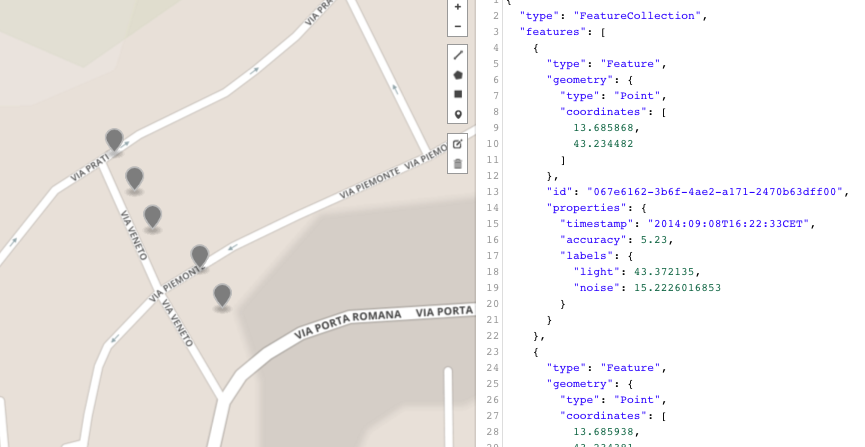
\includegraphics[width=\textwidth]{sample-geojson}
  \caption{\footnotesize{Esempio di visualizzazione GeoJSON relativa ad un invio dati.}}
  \label{fig:sample-geojson}
\end{figure}
Un esempio di contenuto della chiamata è presente all'indirizzo \url{http://path-server.herokuapp.com/public/stub/path-samples.json}. Tale esempio è stato utilizzato anche come traccia condivisa per l'implementazione dell'applicazione \emph{client}. La visualizzazione dei dati inviati può avvenire anche con strumenti esterni che interpretano il formato GeoJSON come presentato in figura \ref{fig:sample-geojson}.

\begin{figure}[ht]
  \centering
  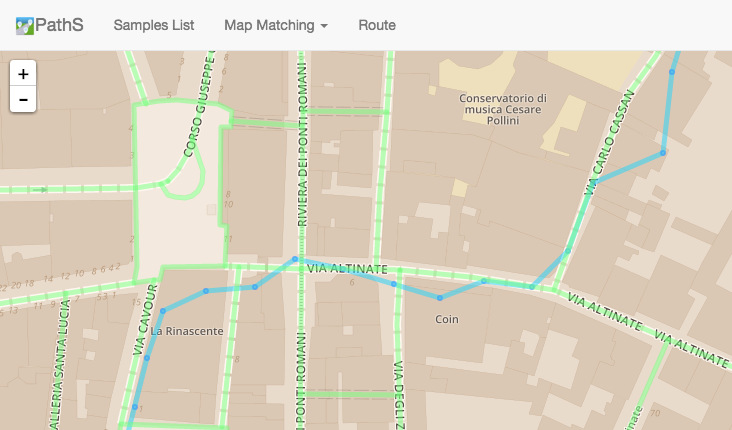
\includegraphics[width=\textwidth]{sample-view}
  \caption{\footnotesize{Esempio di campionamento ricevuto dal server.}}
  \label{fig:sample-view}
\end{figure}

\begin{figure}[ht]
  \centering
  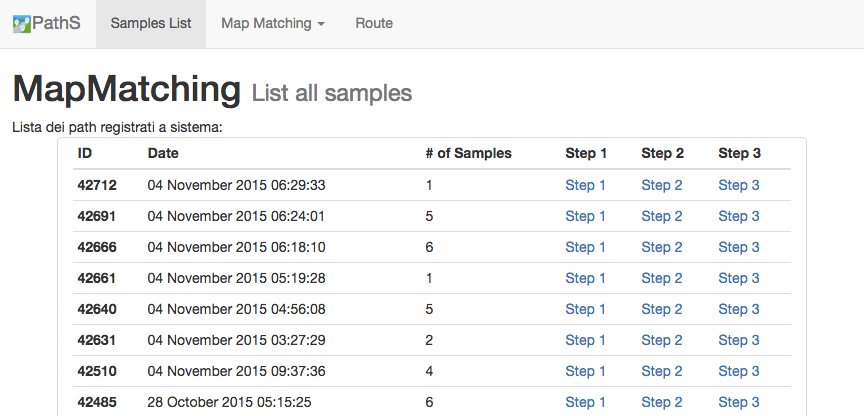
\includegraphics[width=\textwidth]{sample-list}
  \caption{\footnotesize{Lista dei tracciati \emph{Path} ricevuti.}}
  \label{fig:sample-list}
\end{figure}
Il risultato ottenuto dall'invio di alcuni campionamenti al server può essere osservato in figura \ref{fig:sample-view}. Il server mette inoltre a disposizione una pagina di amministrazione che presenta la lista dei traciati ricevuti, le informazioni principali, e i link alla visualizzazione delle altre funzionalità (figura \ref{fig:sample-list}).
